\documentclass{article}
\usepackage{graphicx} % Required for inserting images
\usepackage{authblk}
\usepackage{cite}
\usepackage{natbib}
\usepackage{dcolumn}
\usepackage{pdfpages}
\usepackage{epigraph} % Required for inspirational quote
% packages required for kable()
\usepackage{booktabs}
\usepackage{longtable}
\usepackage{array}
\usepackage{multirow}
\usepackage{wrapfig}
\usepackage{float}
\usepackage{colortbl}
\usepackage{pdflscape}
\usepackage{tabu}
\usepackage{threeparttable}
\usepackage{threeparttablex}
\usepackage[normalem]{ulem}
\usepackage{makecell}
\usepackage{xcolor}
\renewcommand{\epigraphsize}{\small}
\setlength{\epigraphwidth}{0.51\textwidth}
\renewcommand{\textflush}{flushright}
\renewcommand{\sourceflush}{flushright}

% display code
\usepackage{listings}
\usepackage{color}

\definecolor{dkgreen}{rgb}{0,0.6,0}
\definecolor{gray}{rgb}{0.5,0.5,0.5}
\definecolor{mauve}{rgb}{0.58,0,0.82}
\lstset{frame=tb,
  language=Java,
  aboveskip=3mm,
  belowskip=3mm,
  showstringspaces=false,
  columns=flexible,
  basicstyle={\small\ttfamily},
  numbers=none,
  numberstyle=\tiny\color{gray},
  keywordstyle=\color{blue},
  commentstyle=\color{dkgreen},
  stringstyle=\color{mauve},
  breaklines=true,
  breakatwhitespace=true,
  tabsize=3
}


%\date{Draft -- please do not circulate.}

\title{(In)civility on Display: Social Media Discourse through the Ideological Lens}

\author[1]{David Broska}
%\author[2]{Byungkyu Lee}
%\author[3]{Barum Park}
%\author[4]{Daniel A. McFarland}
%\affil[1,4]{Stanford University}
%\affil[2]{New York University}
%\affil[2]{Cornell University}

\begin{document}

\maketitle

\epigraph{Civility costs nothing and buys everything.}{Mary Wortley Montagu 1756}
\epigraph{Civility is on the ballot.}{Barack Obama 2016}
%Respect for women is on the ballot. Tolerance is on the ballot. Justice is on the ballot. Equality is on the ballot. Democracy is on the ballot.

\section{Introduction}

Conversations are at the heart of democracies. Discussions in parliaments, the media, and kitchen tables inform political processes, help identify solutions to problems, avoid violent conflict, and foster a better understanding of each other. Some consider conversations based on reason rather than content and ignorance even a benchmark for achieving a democracy \citep{sanders_against_1997}. Attaining these outcomes requires \textit{civility} from the interlocutors because it sets the stage for productive conversations. 
At a minimum,  civility means ``demonstrating mutual respect" \citep{mutz_inyourface_2016} or ``politeness" \citep{frimer_montagu_2018}. A maximalist definition of civility does not only require being respectful and polite but also critical engagement \citep{kant_enlightenment_1784}\footnote{Kant does not only argue that individuals should not only have the freedom but also the courage to make use of their own understanding -- i.e., to actively engage. For example, the clergyman is required to teach lessons aligned with the ``creed of the church he serves, for he was employed by it on that condition. But as a scholar he has complete freedom and is even called upon to communicate to the public all his carefully examined and well-intentioned thoughts about what is erroneous in that creed and his suggestions for a better arrangement of the religious and ecclesiastical body."} and requires individuals to give rationales in conversation \citep{habermas1985theory}. In other words, this expanded definition of civility demands contributions to conversations to be productive above and beyond avoiding offense.

While this distinction is grounded in theoretical traditions, it remains unclear how these perspectives align with the public's perception of desirable norms in conversations. Civility is a \textit{social praxis} embedded in what people know, who they are, what they do, and what they value. Extant literature does not sufficiently address how the broader public applies norms to conversations, and the social and psychological factors that shape the perceptions of conversations are not well understood. \textit{To what extent does the perception of civility depend on individual factors} (e.g. political ideology, partisanship, age, etc.), \textit{the social context} (e.g. the topic of the conversation), \textit{or both} (e.g. some people in some contexts may perceive conversations differently than others in other contexts)? For this manuscript, we will focus on perceived toxicity, defined as a comment considered disrespectful, hateful, or that makes someone more likely to leave a discussion or give up sharing their perspective. 

This project studies the determinants of perceived civility -- and toxicity in particular -- in the context of the 2016 US presidential election campaign. Across 9,994 conversations held between 2015 and 2017 in political Facebook groups, we study how 4,675 American survey respondents evaluate comments given by discussants in terms of perceived toxicity. The 2016 presidential campaign is an insightful case for the study of conversational norms because the discussions happened ``during a time of rapidly changing norms of political civility" \citep{munger_dont_2021}, and these exchanges were experienced ``first-hand" through broadcasting and online \citep{mutz_inyourface_2016}. Studying social media around this time offers a unique lens into the public sphere because an estimated 68\% of US adults were on a social network, up from 25\% in 2008 \citep{duggan_social_2016}.

%While there was once hope that social media could advance democratic deliberation through open discourse, diverse perspectives, and broad participation, many observers note that social media discussions lack the crucial ingredient of civility. Concerns about declining civility are not new. From the printing press during the Reformation \citep{bejan_mere_2017} to the invention of cable news with its personalized news reporting \citep{mutz_inyourface_2016,berry2014outrage}, history is filled with examples of concerns about incivility of discourse. However, the 2016 US presidential election may have marked another critical turning point in recent history. 

\section{Hypotheses}

\textit{Random intercept hypothesis:} Multilevel models allow for assessing how much variation in perceived toxicity is attributable to survey respondents (e.g. political ideology) and to the context (e.g. the topic of a conversation). We hypothesize that a larger share of the variation in perceived toxicity -- the dependent variable in this study -- is attributable to the context than the individual.

\textit{Individual-level hypothesis:} This study is exploratory and considers a broad range of individual predictors of perceived toxicity. That said, perceptions of conversational norms likely depend on demographic factors such as political ideology, partisanship, education, age, race, and religiosity. These demographics reflect socialization processes that shape what is considered appropriate in a conversation. 

\textit{Context-level hypothesis:} Some topics will be considered more toxic than others. In particular, topics related to ``moral convictions"-- i.e., judgments informed by ``perceptions of morality and immorality, right or wrong" \citep{skitka_conviction_2010} -- may elicit particularly strong reactions. Attitudes toward gun control and abortion may be more strongly held than attitudes toward other issues; these topics may create more intense emotions, motivate people to justify their actions, and lead them to believe that their views are objective and universal. 

\textit{Random slope hypothesis:} Not all comments cause variation in perceived toxicity. Some comments may be irrelevant to the observer, too short to elicit strong reactions, or unintelligible. We hypothesize that the random slopes for individual-level characteristics, coupled with random intercepts for topics, will cover zero. Beyond this, it is interesting to assess the range of the most effects (e.g. 95\%). That is, if the effect for an individual-level characteristic is $\hat \beta$, what is $\beta\pm 1.96$?

\textit{Cross-level interaction hypothesis:} Some topics are perceived as more toxic among Republicans/conservatives than liberals, and vice versa. For example, social identity theory predicts that individuals favor members of the ingroup over the outgroup \citep{tafjelturner_identity_2004}. Hence, Democrats may perceive negative characterizations of Hillary Clinton as more toxic than Republicans. Conversely, Republicans might perceive negative comments about Donald Trump as more toxic than Democrats.






%By highlighting the surveying the dimensions of what constitutes perceptions of a civil discourse, our research informs the literature on content moderation \citep{argyle_leveraging_2023}.


% Social scientists have long observed that “conversation is the soul of democracy” (1, 2). Interpersonal discussions across social divides can help diverse groups of people peacefully identify solutions to shared problems, avoid violent conflict, and come to understand one another better (2–8). Historically, these conversations have occurred face-to-face (8), but online conversations now play a central role in public dialogue. More than 100 billion messages are sent every day on Facebook and Instagram alone (9), and approximately 7 billion conversations occur daily on Facebook Messenger (10). Such conversations can have far-reaching impact. Some of the largest social movements in human history have emerged out of sprawling conversations on social media, and discussions between high-profile social media users can shape the stock market, politics, and many other aspects of human experience (11–14). The internet thus has the capacity to empower an ever-increasing number of people to communicate and deliberate together

\section{Data}

To study the determinants of perceived civility in conversations, we recruit 4,675 American adults via Prolific to fill out a survey asking them to evaluate Facebook conversations regarding perceived toxicity and other features. Respondents who did not pass an attention check were not allowed to take the survey. Excluding missing values\footnote{There is no evidence of differential attrition.}, the total sample size is 32,597 observations. Those who passed the attention check were randomly assigned to evaluate 7 conversations. Not every respondent evaluated each conversation; each one was evaluated 3.27 times on average. 

The 9,994 conversations are a stratified random sample of conversations from 1,058 public Facebook pages retrieved during the 2016 US presidential campaign via the official Facebook API v2.7. To ensure variation across the ideological spectrum on Facebook, we first obtained a list of the 500 most active political pages of the platform according to \citet{bakshy_exposure_2015}, as well as 37 pages identified as representative online and offline news sources by Pew Research Center’s American Trends Panel in 2014. These pages make up our media samples.

Table \ref{tab:summ-tab-ind} in the Supplementary Material provides summary statistics of the characteristics of survey respondents. Compared to demographic quotas from the American National Election Studies (ANES), this sample of 4,675 adults recruited via Prolific consists of more college-educated individuals (+10.7 percentage points) than those with a high school degree or less (-7.3pp). We over-sampled Democrats (+10.7pp) and under-sampled Republicans (-14.6pp). Finally, we over-sampled those aged 33 to 44 (+9.4pp), and under-sampled those aged 60 and older (-12.3pp). The sample is otherwise representative on these demographic dimensions. In a future analysis, we will consider whether results change if post-stratification techniques are applied, allowing us to make more credible inferences about the population of American adults.


Table \ref{tab:summ-tab-topics} provides summary statistics of variables measured for conversations; the first set of variables in the \textit{Topic} category refers to categorizations of whether a particular comment is related to a topic or not. The Facebook comments were classified with a Large Language Model (LLM) to create predictor variables for the regression analysis (please refer to Figure \ref{fig:intercoder-reliability} for more details). The \textit{Other} variables denote predictors unrelated to the language of the comment.

%\begin{itemize}
%    \item \textit{Order:} how many conversations a respondent evaluate before rating the focal one
%    \item \textit{BToxicNum01:} toxicity of B's comment rated by survey respondents. The four levels Not Toxic (-1), Maybe not sure (0), Toxic (1), and Very toxic (2) were rescaled to range from 0 to 1 and will be treated as a continuous dependent variable.
%    \item \textit{ideocommenterB}: the political ideology of commenter B is estimated based on the Facebook pages that the user visited. Negative values denote liberal political ideology while positive values represent conservatism.
%\end{itemize}

Table \ref{tab:summ-tab-emf} shows summary statistics on sentiment scores assigned to commenter B's comment assigned with the expanded Moral Foundations Dictionary \citep{hopp2021extended}.\footnote{"Each word is assigned 5 sentiment scores that denote the average sentiment of the foundation context in which this word appeared. For example, the word 'kill' has an average 'care_sent' of -0.69, meaning that all 'care-harm' highlights in which 'kill' appeared had an average, negative sentiment of -0.69." 

https://github.com/medianeuroscience/emfdscore/blob/master/eMFDscore_Tutorial.ipynb}
Table \ref{tab:summ-tab-liwc} presents the word frequencies per category in the LIWC dictionary \citep{pennebaker_linguistic_2022}. The counts were transformed with $\log(1+x)$ to account for the right-skew of count variables. These dictionary counts will be included as control variables but they do not represent the focus of the analysis.

\section{Methods}

Multilevel models, also known as mixed-effects models, are statistical models used for analyzing data that have a nested structure (see Table \ref{sample-table}  for illustration). This means that the data is organized into groups, and there is variability both within each group and between groups \citep{hox2017multilevel}. Multilevel models can account for correlation within each group. In the present case, evaluations of conversations may be correlated within each individual (because it is the same rater), and conversations may be evaluated similarly (because it is the entity). This does not imply a strictly hierarchical structure since each respondent evaluated multiple conversations but not all conversations have been evaluated by the same respondents. Hence, these data are cross-classified.

\section{Results}

In the following, I will refer to the models reported in the table on pp.13.

\textit{Random intercept hypothesis:} The intraclass correlation indicates that approximately 11\% of the variation in perceived toxicity is attributable to individual factors whereas 39\% of the variation comes from features of the comments (see Model 1). 

\textit{Individual-level hypothesis:} Several individual-level predictors are associated with perceived toxicity. For example, a 2 standard deviation increase in political ideology -- i.e., an increase of approximately 3.5 points on a 1 to 7 scale corresponding to a shift from extremely liberal to moderate or from moderate to extremely conservative -- is associated with an approximate decrease of 6 percentage points in average perceived toxicity, controlling for other variables in the model. More broadly, this association suggests that liberals are more sensitive while conservatives are less so. The magnitude of this association is comparable to a 20-year increase in age. While older folks tend to be less sensitive, more educated people tend to rate comments as more toxic on average. Finally, the coefficient for \textit{Order} suggests that processes by which people get numbed partially explain insensitivity. Having been exposed to six comments before rating the 7th is comparable to the magnitude of the association with political ideology. In total, the individual-level predictors in Model 2 explain 9\% of the variance at the individual level -- i.e. 9\% of 11\%.

\textit{Context-level hypothesis:} The comments on the following topics are considered significantly more toxic (example Facebook comments in parenthesis): 
\begin{itemize}
    \item Negative characterization of America (e.g. ``The US is governed by incompetent politicians")
    \item Suggestive content (e.g. ``Prostitutes will be like ...")
    \item Negative characterization of Hillary Clinton (e.g. ``Hillary is a liar and she will never be president of the United States")
    \item Drugs (e.g. ``She's high on drugs of stupidity", ``And who's fault is it that the cartels exist?? Your people")
    \item Negative characterization of immigrants (e.g. ``The immigrants steal our jobs")
\end{itemize}

Only two topics are perceived as significantly less toxic on average.

\begin{itemize}
    \item Positive characterization of Hillary Clinton (e.g. ``During the debates, Hillary will mop Donald Trump off of the floor and him into the sewer because she is 20x smarter")
    \item Positive characterization of immigrants (e.g. ``Most immigrants are actually highly educated doctors, lawyers, and computer engineers")
\end{itemize}

Comparing the a model only with random intercepts against model that also includes the topic predictors (not shown in table), we find that including the 14 topics explains about 13.7\% of the variance in perceived toxicity at the conversation level -- i.e. 13.7\% of the 39\%. 



\textit{Random slope hypothesis:} According to model 4,\footnote{Model 4 did not converge when using both random slopes and control variables.} the standard deviation of the random slopes for political ideology estimated for each comment is 0.085. Based on this, we estimate that 95\% of the slopes are between $-0.065 - 1.96\times 0.085=-0.23$ and  $-0.0645 + 1.96 \times 0.085=0.10$. In line with our hypothesis above, this means that the relationship between political and perceived toxicity is zero for some comments. In other words, some comments do not elicit a reaction across the ideological spectrum. These comments might be too short, unintelligible, or uncontroversial.

\textit{Cross-level interaction hypothesis:} Model 5 estimates interactions effects. For a given topic, a negative effect means that conservatives perceive a comment as less toxic than liberals. Conservatives find comments that endorse abortion, immigration, Hillary Clinton, and that characterize Trump negatively significantly more toxic than liberals. Conservatives perceive comments related to anti-America rhetoric, pro-Trump, anti-Clinton, and anti-abortion as less toxic. In sum, I find support for the hypothesis that the association between political ideology and perceived toxicity depends on the topic. These interaction effects were estimated in a single model. Estimates from separate models are very similar in terms of the sign and statistical significance of the coefficients (see Table \ref{tab:interaction-effects-comparison}).

\section{Conclusion and Discussion}

Conversations are a crucial element in the democratic process. If someone perceives a conversation as toxic, they might be reluctant to share their perspective or disengage altogether. This study offers preliminary results on the determinants of perceived toxicity in conversations. We find that more variation in perceived toxicity is attributable to the features of comments than to individual-level factors (approximately 3.5 times more variation). Across comments, liberals are more sensitive than conservatives, and this effect seems sizable compared to other predictors' effects. Why are conservatives less sensitive? On average, conservatives have been exposed to more irritating content on social media more often than liberals. For example, \citet{bakshy_exposure_2015} find that conservatives encounter more content that cuts across ideological lines than liberals through friends, their user feed, and the content they click on. That said, the relationship between political ideology and perceived toxicity is not uniform. Both conservatives and liberals are more sensitive when it comes to certain issues. In line with social identity theory, for instance, liberals perceive negative comments on Hillary Clinton as more toxic and conservatives are more sensitive towards negative portrayals of Donald Trump. 

While these results are promising, we would be remiss not to mention this work's shortcomings. Toxicity is only one dimension of civility and similar analyses can be conducted for other dependent variables in this dataset, including perceived hate speech or perceived productivity of a conversation. A similar point can be made about the independent variables in this study; many more deserve closer attention than was given in this short report. Last, this analysis has raised more questions than it provides answers. What are the social and psychological processes that underlie differences in perceived toxicity between liberals and conservatives? We will address this question in an expanded version of this research project. 

\newpage
\bibliographystyle{asr}
\bibliography{bib}

\clearpage
\section{Supplementary Material}

\begin{table}[htbp]
    \centering
    \begin{tabular}{|c|c|c|c|}
    \hline
    \textbf{Respondent Id} & \textbf{Post Id} & \textbf{Comment A Id} & \textbf{Comment B Id} \\
    \hline
    R1 & P2 & A2 & B2 \\
    R1 & P13 & A13 & B13 \\
    R1 & P23 & A23 & B23 \\
    R1 & P5 & A5 & B5 \\
    R1 & P6 & A6 & B6 \\
    R1 & P56 & A56 & B56 \\
    \midrule
    R2 & P4 & A4 & B4 \\
    R2 & P3 & A3 & B3 \\
    R2 & P8 & A8 & B8 \\
    R2 & P9 & A9 & B9 \\
    R2 & P10 & A10 & B10 \\
    R2 & P11 & A11 & B11 \\
    R2 & P12 & A12 & B12 \\
    \midrule
    R3 & P6 & A6 & B6 \\
    R3 & P22 & A22 & B22 \\
    R3 & P4 & A4 & B4 \\
    R3 & P7 & A7 & B7 \\
    R3 & P9994 & A9994 & B9994 \\
    R3 & P11 & A11 & B11 \\
    R3 & P55 & A55 & B55 \\
    \dots & \dots & \dots & \dots \\
    \hline
    \end{tabular}
    \caption{Sample table to illustrate the nested data structure}
    \label{sample-table}
\end{table}

\clearpage

% Dependent variable plot 

\begin{figure}[h]
    \centering
    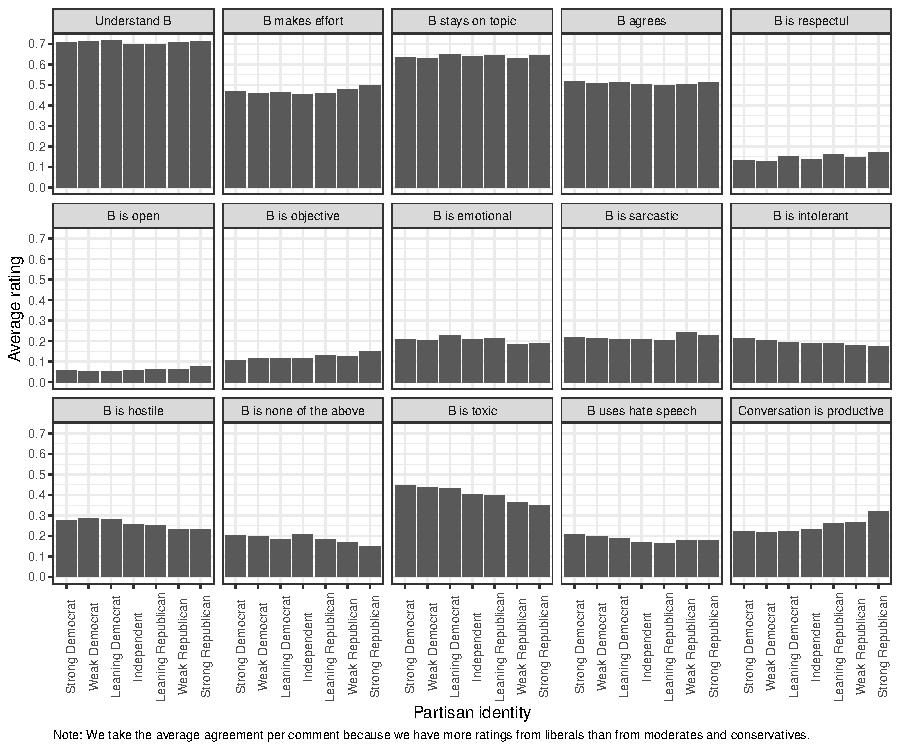
\includegraphics[width=1\linewidth]{figures/2_AvgAgreement_Partisanship.pdf}
    \caption{Variables measuring dimensions of civility by partisanship}
    \label{fig:civility-partisanship}
    \vspace{0.25cm}
    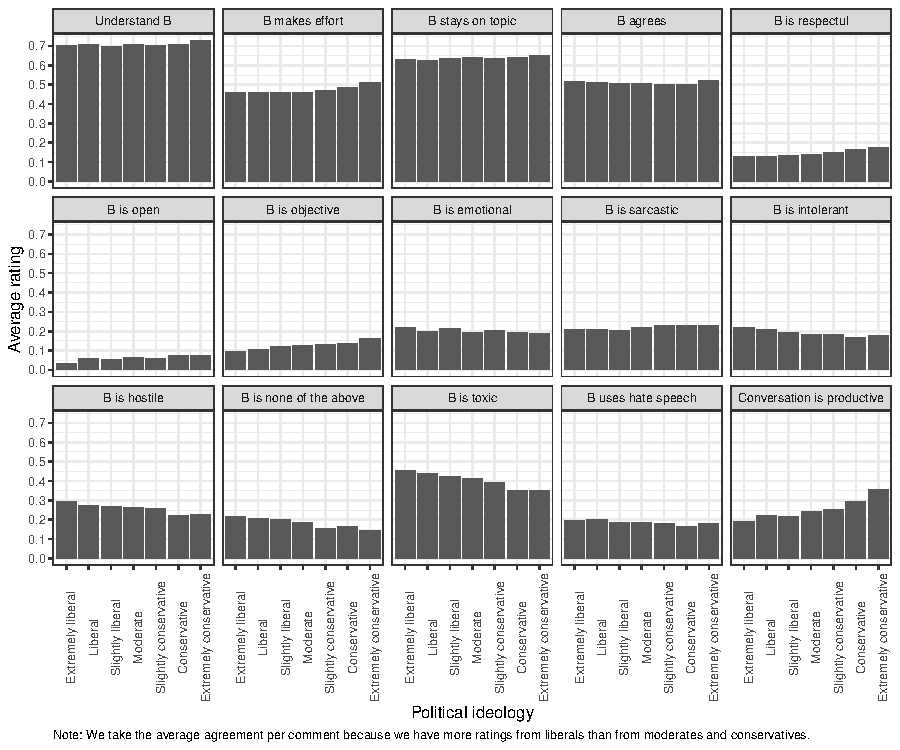
\includegraphics[width=1\linewidth]{figures/2_AvgAgreement_Ideo.pdf}
    \caption{Variables measuring dimensions of civility by political ideology}
    \label{fig:civility-ideology}
\end{figure}
\clearpage
%%%%%%%%%%%%%%%%%%%%%%%%%%%%%%%%%%%%%%%%%%
% Summary statistics % 
\renewcommand{\arraystretch}{0.9}
\begin{table}[!h]
\centering
\caption{\label{tab:summ-tab-ind}Summary statistics on characteristics of survey respondents}
\centering
\begin{tabular}[t]{llrrrrrr}
\toprule
Type & Variable & Min & Q25 & Mean & Median & Q75 & Max\\
\midrule
Dependent Variable & BToxicNum01 & -0.42 & -0.42 & 0.00 & -0.08 & 0.25 & 0.58\\
\cmidrule{1-8}
 & PolIdComp & 1.00 & 1.50 & 3.18 & 3.00 & 4.50 & 7.00\\
\cmidrule{2-8}
 & PolIdComp2Sd & -0.61 & -0.47 & 0.00 & -0.05 & 0.37 & 1.07\\
\cmidrule{2-8}
 & Man & 0.00 & 0.00 & 0.49 & 0.00 & 1.00 & 1.00\\
\cmidrule{2-8}
 & Woman & 0.00 & 0.00 & 0.48 & 0.00 & 1.00 & 1.00\\
\cmidrule{2-8}
 & OtherGender & 0.00 & 0.00 & 0.02 & 0.00 & 0.00 & 1.00\\
\cmidrule{2-8}
 & EducationNum & 1.00 & 3.00 & 3.05 & 3.00 & 3.00 & 5.00\\
\cmidrule{2-8}
 & Income2Sd & -0.58 & -0.30 & 0.00 & -0.13 & 0.38 & 1.79\\
\cmidrule{2-8}
 & Asian & 0.00 & 0.00 & 0.07 & 0.00 & 0.00 & 1.00\\
\cmidrule{2-8}
 & Black & 0.00 & 0.00 & 0.15 & 0.00 & 0.00 & 1.00\\
\cmidrule{2-8}
 & Hispanic & 0.00 & 0.00 & 0.08 & 0.00 & 0.00 & 1.00\\
\cmidrule{2-8}
 & White & 0.00 & 1.00 & 0.76 & 1.00 & 1.00 & 1.00\\
\cmidrule{2-8}
 & OtherRace & 0.00 & 0.00 & 0.03 & 0.00 & 0.00 & 1.00\\
\cmidrule{2-8}
 & Married & 0.00 & 0.00 & 0.39 & 0.00 & 1.00 & 1.00\\
\cmidrule{2-8}
 & Separated & 0.00 & 0.00 & 0.01 & 0.00 & 0.00 & 1.00\\
\cmidrule{2-8}
 & Widowed & 0.00 & 0.00 & 0.02 & 0.00 & 0.00 & 1.00\\
\cmidrule{2-8}
 & MaritalNoAnswer & 0.00 & 0.00 & 0.02 & 0.00 & 0.00 & 1.00\\
\cmidrule{2-8}
 & Divorced & 0.00 & 0.00 & 0.10 & 0.00 & 0.00 & 1.00\\
\cmidrule{2-8}
 & NeverMarried & 0.00 & 0.00 & 0.46 & 0.00 & 1.00 & 1.00\\
\cmidrule{2-8}
 & EvangelicalProtestant & 0.00 & 0.00 & 0.11 & 0.00 & 0.00 & 1.00\\
\cmidrule{2-8}
 & MainlineProtestant & 0.00 & 0.00 & 0.11 & 0.00 & 0.00 & 1.00\\
\cmidrule{2-8}
 & Mormon & 0.00 & 0.00 & 0.01 & 0.00 & 0.00 & 1.00\\
\cmidrule{2-8}
 & Catholic & 0.00 & 0.00 & 0.16 & 0.00 & 0.00 & 1.00\\
\cmidrule{2-8}
 & Jewish & 0.00 & 0.00 & 0.02 & 0.00 & 0.00 & 1.00\\
\cmidrule{2-8}
 & Muslim & 0.00 & 0.00 & 0.01 & 0.00 & 0.00 & 1.00\\
\cmidrule{2-8}
 & NotReligious & 0.00 & 0.00 & 0.00 & 0.00 & 0.00 & 0.00\\
\cmidrule{2-8}
 & ReligionNoAnswer & 0.00 & 0.00 & 0.00 & 0.00 & 0.00 & 0.00\\
\cmidrule{2-8}
\multirow{-27}{*}{\raggedright\arraybackslash Demographics} & OtherReligion & 0.00 & 0.00 & 0.09 & 0.00 & 0.00 & 1.00\\
\bottomrule
\end{tabular}
\end{table}


\begin{table}[!h]
\centering
\caption{\label{tab:summ-tab-topics}Summary statistics on conversation characteristics (1). LIWC}
\centering
\begin{tabular}[t]{llrrrrrr}
\toprule
Type & Variable & Min & Q25 & Mean & Median & Q75 & Max\\
\midrule
 & antiamerica & 0.00 & 0.00 & 0.13 & 0.00 & 0.00 & 1.00\\
\cmidrule{2-8}
 & antichristianity & 0.00 & 0.00 & 0.00 & 0.00 & 0.00 & 1.00\\
\cmidrule{2-8}
 & suggestive & 0.00 & 0.00 & 0.12 & 0.00 & 0.00 & 1.00\\
\cmidrule{2-8}
 & drugs & 0.00 & 0.00 & 0.02 & 0.00 & 0.00 & 1.00\\
\cmidrule{2-8}
 & antitrump & 0.00 & 0.00 & 0.11 & 0.00 & 0.00 & 1.00\\
\cmidrule{2-8}
 & protrump & 0.00 & 0.00 & 0.05 & 0.00 & 0.00 & 1.00\\
\cmidrule{2-8}
 & anticlinton & 0.00 & 0.00 & 0.12 & 0.00 & 0.00 & 1.00\\
\cmidrule{2-8}
 & proclinton & 0.00 & 0.00 & 0.02 & 0.00 & 0.00 & 1.00\\
\cmidrule{2-8}
 & antiimmigrant & 0.00 & 0.00 & 0.12 & 0.00 & 0.00 & 1.00\\
\cmidrule{2-8}
 & proimmigrant & 0.00 & 0.00 & 0.01 & 0.00 & 0.00 & 1.00\\
\cmidrule{2-8}
 & antiabortion & 0.00 & 0.00 & 0.01 & 0.00 & 0.00 & 1.00\\
\cmidrule{2-8}
 & proabortion & 0.00 & 0.00 & 0.01 & 0.00 & 0.00 & 1.00\\
\cmidrule{2-8}
 & antigun & 0.00 & 0.00 & 0.00 & 0.00 & 0.00 & 1.00\\
\cmidrule{2-8}
 & progun & 0.00 & 0.00 & 0.01 & 0.00 & 0.00 & 1.00\\
\cmidrule{2-8}
\multirow{-15}{*}{\raggedright\arraybackslash Topic} & antiwhite & 0.00 & 0.00 & 0.05 & 0.00 & 0.00 & 1.00\\
\cmidrule{1-8}
 & Order & -3.00 & -2.00 & 0.00 & 0.00 & 2.00 & 3.00\\
\cmidrule{2-8}
 & IdeoCommenterB & -0.96 & -0.37 & 0.14 & 0.14 & 0.76 & 1.01\\
\cmidrule{2-8}
\multirow{-3}{*}{\raggedright\arraybackslash Other} & TargetLikesCount & 0.00 & 0.00 & 0.53 & 0.00 & 0.69 & 7.18\\
\bottomrule
\end{tabular}
\end{table}


\begin{table}[!h]
\centering
\caption{\label{tab:summ-tab-emf}Summary statistics on conversation characteristics (2). Moral foundations dictionary}
\centering
\begin{tabular}[t]{llrrrrrr}
\toprule
Type & Variable & Min & Q25 & Mean & Median & Q75 & Max\\
\midrule
 & CareNegSen2Sd & -6.38 & -0.22 & 0 & -0.08 & 0.17 & 5.67\\
\cmidrule{2-8}
 & FairnessNegSen2Sd & -7.12 & -0.17 & 0 & -0.10 & 0.13 & 5.80\\
\cmidrule{2-8}
 & LoyaltyNegSen2Sd & -5.56 & -0.18 & 0 & -0.10 & 0.12 & 6.58\\
\cmidrule{2-8}
 & AuthorityNegSen2Sd & -5.39 & -0.17 & 0 & -0.10 & 0.14 & 5.97\\
\cmidrule{2-8}
\multirow{-5}{*}{\raggedright\arraybackslash Moral Foundations} & SanctityNegSen2Sd & -5.68 & -0.18 & 0 & -0.09 & 0.16 & 6.18\\
\bottomrule
\end{tabular}
\end{table}

\begin{table}[!h]
\centering
\caption{\label{tab:summ-tab-liwc}Summary statistics on conversation characteristics (3)}
\centering
\begin{tabular}[t]{llrrrrrr}
\toprule
Type & Variable & Min & Q25 & Mean & Median & Q75 & Max\\
\midrule
 & tone\_pos & 0 & 0 & 0.62 & 0.00 & 1.30 & 4.62\\
\cmidrule{2-8}
 & tone\_neg & 0 & 0 & 1.03 & 0.00 & 2.13 & 4.62\\
\cmidrule{2-8}
 & emo\_pos & 0 & 0 & 0.20 & 0.00 & 0.00 & 4.62\\
\cmidrule{2-8}
 & emo\_neg & 0 & 0 & 0.22 & 0.00 & 0.00 & 4.62\\
\cmidrule{2-8}
 & swear & 0 & 0 & 0.54 & 0.00 & 0.00 & 4.62\\
\cmidrule{2-8}
 & conflict & 0 & 0 & 0.18 & 0.00 & 0.00 & 4.62\\
\cmidrule{2-8}
 & prosocial & 0 & 0 & 0.15 & 0.00 & 0.00 & 4.62\\
\cmidrule{2-8}
 & polite & 0 & 0 & 0.12 & 0.00 & 0.00 & 4.62\\
\cmidrule{2-8}
 & moral & 0 & 0 & 0.36 & 0.00 & 0.00 & 4.62\\
\cmidrule{2-8}
 & comm & 0 & 0 & 0.28 & 0.00 & 0.00 & 4.62\\
\cmidrule{2-8}
 & cogproc & 0 & 0 & 1.62 & 2.16 & 2.77 & 4.62\\
\cmidrule{2-8}
 & politic & 0 & 0 & 0.39 & 0.00 & 0.00 & 4.62\\
\cmidrule{2-8}
 & ethnicity & 0 & 0 & 0.25 & 0.00 & 0.00 & 4.62\\
\cmidrule{2-8}
 & tech & 0 & 0 & 0.19 & 0.00 & 0.00 & 4.62\\
\cmidrule{2-8}
 & leisure & 0 & 0 & 0.07 & 0.00 & 0.00 & 4.62\\
\cmidrule{2-8}
 & home & 0 & 0 & 0.07 & 0.00 & 0.00 & 3.93\\
\cmidrule{2-8}
 & work & 0 & 0 & 0.23 & 0.00 & 0.00 & 3.93\\
\cmidrule{2-8}
 & money & 0 & 0 & 0.15 & 0.00 & 0.00 & 3.93\\
\cmidrule{2-8}
 & relig & 0 & 0 & 0.19 & 0.00 & 0.00 & 4.62\\
\cmidrule{2-8}
 & substances & 0 & 0 & 0.01 & 0.00 & 0.00 & 3.93\\
\cmidrule{2-8}
 & sexual & 0 & 0 & 0.19 & 0.00 & 0.00 & 4.62\\
\cmidrule{2-8}
 & food & 0 & 0 & 0.08 & 0.00 & 0.00 & 4.21\\
\cmidrule{2-8}
 & death & 0 & 0 & 0.10 & 0.00 & 0.00 & 3.93\\
\cmidrule{2-8}
 & male & 0 & 0 & 0.28 & 0.00 & 0.00 & 4.62\\
\cmidrule{2-8}
 & female & 0 & 0 & 1.04 & 0.00 & 2.40 & 4.62\\
\cmidrule{2-8}
 & shehe & 0 & 0 & 0.75 & 0.00 & 1.83 & 4.62\\
\cmidrule{2-8}
 & they & 0 & 0 & 0.35 & 0.00 & 0.00 & 3.93\\
\cmidrule{2-8}
 & you & 0 & 0 & 0.52 & 0.00 & 0.00 & 4.62\\
\cmidrule{2-8}
 & i & 0 & 0 & 0.42 & 0.00 & 0.00 & 4.62\\
\cmidrule{2-8}
 & we & 0 & 0 & 0.23 & 0.00 & 0.00 & 3.93\\
\cmidrule{2-8}
 & Emoji & 0 & 0 & 0.03 & 0.00 & 0.00 & 6.22\\
\cmidrule{2-8}
 & power & 0 & 0 & 0.60 & 0.00 & 1.35 & 4.62\\
\cmidrule{2-8}
\multirow{-33}{*}{\raggedright\arraybackslash LIWC} & achieve & 0 & 0 & 0.21 & 0.00 & 0.00 & 4.62\\
\bottomrule
\end{tabular}
\end{table}

\clearpage
% End summary statistics 
%%%%%%%%%%%%%%%%%%%%%%%%%%%%%%%%%%%%%%%%%%%%



% Regression table 
\clearpage
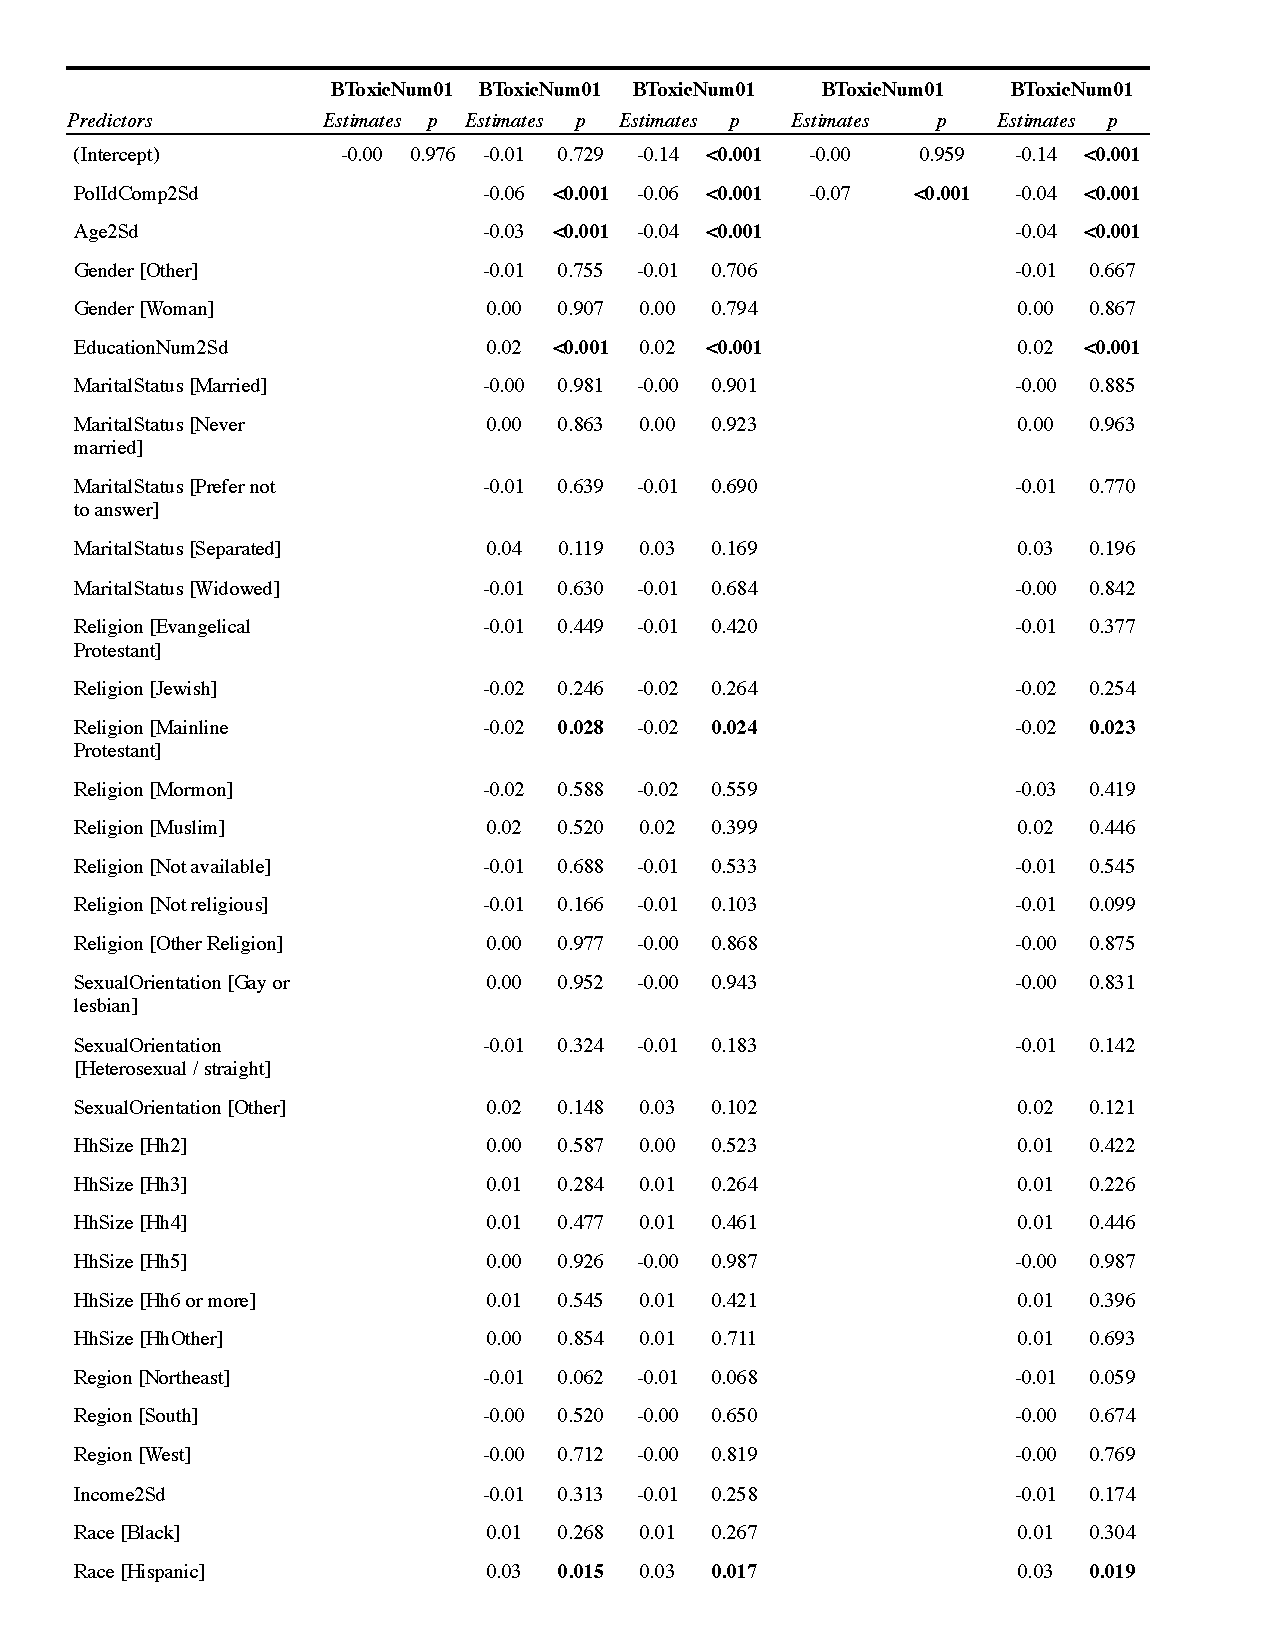
\includepdf[pages={1-},scale=0.95]{tox.html.pdf}




% Model comparison interaction effects

The interaction effects reported in the main text were estimated with a single model. To assess the robustness of these results, these effects were also estimated with separate models. Table \ref{tab:interaction-effects-comparison} shows that in all but four cases the interaction effects estimates had the sign and were either both significant or both insignificant. Additionally, in all but one case (\textit{antitrump}), the effects had the same sign.

\begin{table}[!h]
\centering
\caption{\label{tab:interaction-effects-comparison}Comparing interaction effects estimated with separate models to those estimated with a single model}
\centering
\begin{tabular}[t]{lrrrlll}
\toprule
Term & Seperate & Single model & Sign & Significance & Consistent & Difference\\
\midrule
PolIdComp2Sd:protrump & -0.10 & -0.05 & -0.05 & Yes & Yes & Yes\\
\cmidrule{1-7}
PolIdComp2Sd:antiamerica & -0.05 & -0.02 & -0.03 & Yes & Yes & Yes\\
\cmidrule{1-7}
PolIdComp2Sd:antichristianity & -0.03 & 0.00 & -0.03 & Yes & Yes & Yes\\
\cmidrule{1-7}
PolIdComp2Sd:antigun & 0.01 & 0.03 & -0.02 & Yes & Yes & Yes\\
\cmidrule{1-7}
PolIdComp2Sd:IdeoCommenterB2Sd & -0.08 & -0.06 & -0.02 & Yes & Yes & Yes\\
\cmidrule{1-7}
PolIdComp2Sd:antiimmigrant & -0.11 & -0.09 & -0.02 & Yes & Yes & Yes\\
\cmidrule{1-7}
PolIdComp2Sd:anticlinton & -0.07 & -0.06 & -0.02 & Yes & Yes & Yes\\
\cmidrule{1-7}
PolIdComp2Sd:proabortion & 0.10 & 0.10 & -0.01 & Yes & Yes & Yes\\
\cmidrule{1-7}
PolIdComp2Sd:TargetLikesCount2Sd & 0.00 & -0.01 & 0.01 & Yes & Yes & Yes\\
\cmidrule{1-7}
PolIdComp2Sd:proclinton & 0.04 & 0.04 & 0.01 & Yes & Yes & Yes\\
\cmidrule{1-7}
PolIdComp2Sd:EducationNum2Sd & 0.01 & 0.00 & 0.00 & Yes & Yes & Yes\\
\cmidrule{1-7}
PolIdComp2Sd:Income2Sd & 0.01 & 0.01 & 0.00 & Yes & Yes & Yes\\
\cmidrule{1-7}
PolIdComp2Sd:Order2Sd & -0.01 & 0.00 & 0.00 & Yes & Yes & Yes\\
\cmidrule{1-7}
PolIdComp2Sd:Age2Sd & 0.00 & 0.00 & 0.00 & Yes & Yes & Yes\\
\cmidrule{1-7}
PolIdComp2Sd:suggestive & -0.01 & -0.01 & 0.00 & Yes & Yes & Yes\\
\cmidrule{1-7}
PolIdComp2Sd:drugs & -0.02 & -0.02 & 0.00 & Yes & Yes & Yes\\
\cmidrule{1-7}
PolIdComp2Sd:antitrump & -0.01 & 0.04 & -0.05 & No & No & No\\
\cmidrule{1-7}
PolIdComp2Sd:progun & -0.09 & -0.06 & -0.04 & Yes & No & No\\
\cmidrule{1-7}
PolIdComp2Sd:proimmigrant & 0.04 & 0.06 & -0.03 & Yes & No & No\\
\cmidrule{1-7}
PolIdComp2Sd:antiabortion & -0.04 & -0.06 & 0.02 & Yes & No & No\\
\bottomrule
\end{tabular}
\end{table}

\clearpage

\clearpage

\begin{figure}[h]
    \centering
    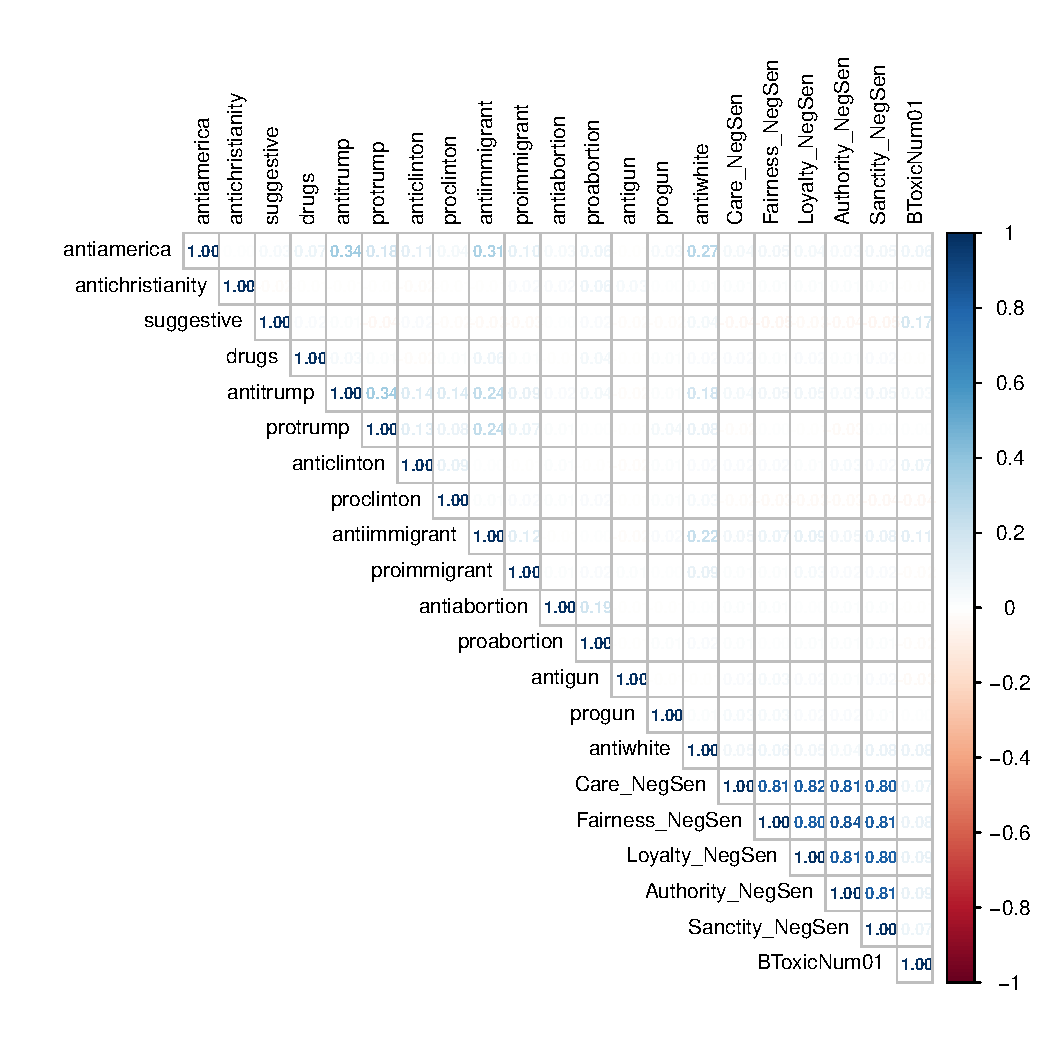
\includegraphics[width=1\linewidth]{figures/corrplot_topics.pdf}
    \caption{Correlation plot. The small Pearson correlations between topics indicate that topics capture distinct dimensions with little overlap. This occurs because most comments are short, communicating only one or few issues.}
    \label{fig:corrplot-topics}
\end{figure}
\clearpage

% Intercoder reliability
\begin{figure}
    \centering
    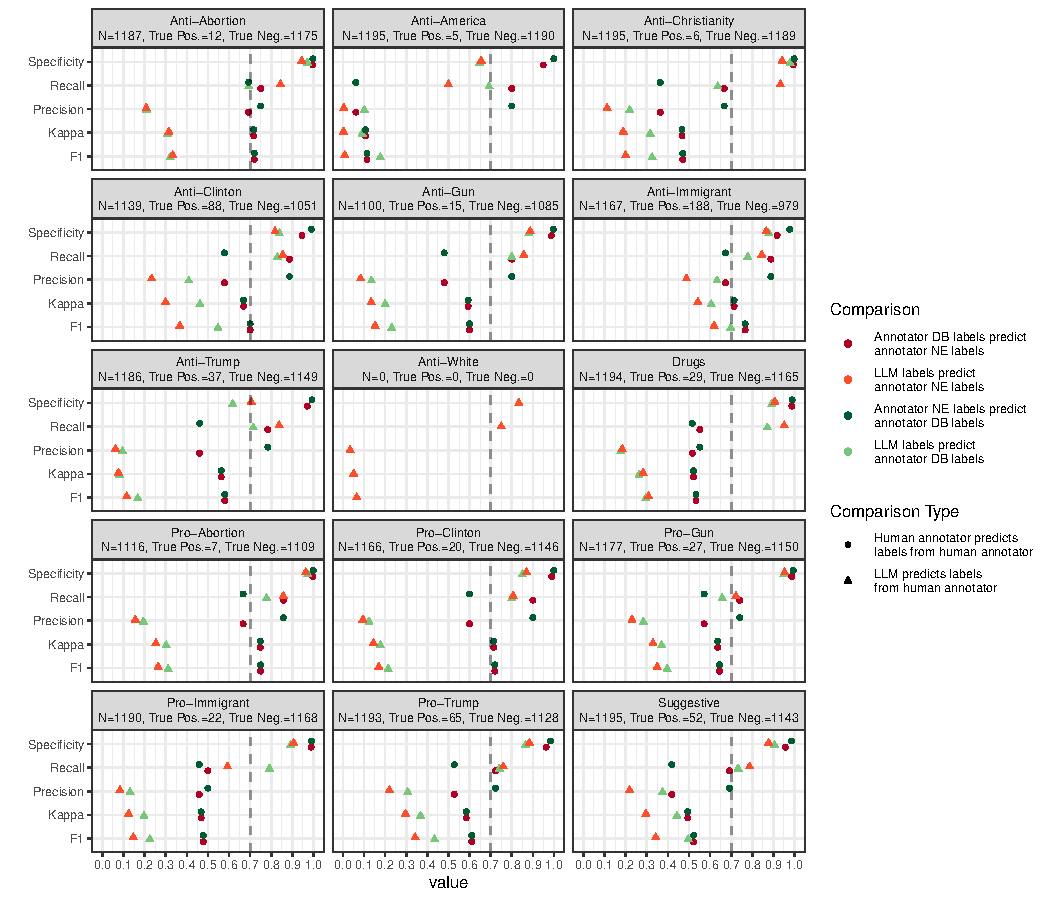
\includegraphics[width=1.3\linewidth]{figures/classifier_performance.pdf}
    \caption{Inter-coder reliability for classifying a comment as either relevant or irrelevant to a topic. Reliability is calculated for two human annotators and one LLM (Mistral 8GB). For example, the dark green dots indicate reliability when human annotator DB is considered the 'ground truth'., and these annotated labels are predicted by the LLM (light green) or the human annotators NE (dark red). In general, the LLM accurately identifies comments irrelevant to a topic (near-perfect specificity) and delivers acceptable performance in identifying all relevant comments (recall). The LLM does not perform well at discerning between relevant and irrelevant comments -- i.e., avoiding false positives (low precision). Given the small number of true positives, we will manually label all cases labeled as relevant by the LLM, thereby maximizing specificity.}
    \label{fig:intercoder-reliability}
\end{figure}
\clearpage

%\subsection{Drugs}

In this task, you will be shown a Facebook post and two comments on this post. One comment is from person A and the other comment is from person B. 
    
Your job is to determine if the comment by B is related to the consumption, production, or distribution of drugs. Drugs refer to substances with psychoactive effects. 

Your answer must be a single number: 0 if irrelevant, 1 if relevant.

Here are some examples with reasoning. Use the following format for your output:

Example 1:
Comment by B: "She is high on drugs of stupidity!"
Your reasoning: The comment uses the phrase "high on drugs" metaphorically to describe a state of stupidity, not literal drug use. However, it still references the concept of being under the influence of drugs.
Your answer: 1

Example 2:
Comment by B: "And who's fault is it that the cartels exist ?? Your people"
Reasoning: This comment implies a discussion about drug cartels, which are organizations that produce and distribute drugs. Therefore, it is relevant to the topic of drugs.
Your answer: 1

Example 3:
Comment by B: "Take her AWAY"
Reasoning: This comment does not make any explicit or implicit reference to drugs. Hence, the comment is irrelevant to the topic of drugs.
Your answer: 0


\subsection{Suggestive content}

 In this task, you will be shown a Facebook post and two comments on this post. One comment is from person A and the other comment is from person B. 
    
Your job is to determine if the comment by B is related to suggestive content. Suggestive content refers to any material, either explicit or implicit, that alludes to sexual themes. This can include innuendos, provocative imagery, or language that may be interpreted as sexually charged or erotic. 

Your answer must be a single number: 0 if irrelevant, 1 if relevant.

Here are some examples with reasoning. Use the following format for your output:

Example 1:
Comment by B: "If those prostitutes have balls."
Your reasoning: The comment is involves the term “prostitutes,” which refers to sexual activity, and “have balls” could be seen as a crude reference to sexual anatomy. Hence, it is relevant to suggestive content.
Your answer: 1

Example 2:
Comment by B: "They have hunting... And dicks on their brain!"
Reasoning: The term "dicks" is a sexual reference. Thus, this comment involves suggestive content.
Your answer: 1

Example 3:
Comment by B: "Very painful to watch."
Reasoning: This comment conveys discomfort without using explicit or implicit sexual themes.
Your answer: 0

    
    
\subsection{Negative portrayal of Christianity}

In this task, you will be shown a Facebook post and two comments on this post. One comment is from person A and the other comment is from person B. 
    
Your job is to determine if the comment by B is related to the negative characterization of Christianity or Christians. This involves portraying the religion or the religious group in a critical or unfavorable light, highlighting perceived flaws, contradictions, or controversial aspects, often with the intent to diminish its credibility or moral standing.

Your answer must be a single number: 0 if irrelevant, 1 if relevant.

Here are some examples with reasoning. Use the following format for your output:

Example 1:
Comment by B: "Another good 'Christian' pedophile!"
Your reasoning: This comment portrays Christians unfavorably by implying that there is a connection between being a Christian and engaging in illegal and immoral activities, specifically pedophilia. 
Your answer: 1

Example 2:
Comment by B: "Don't tell Muslim terrors because all Christian terror everyday kill 1000 children in Syria"
Reasoning: This comment characterizes Christianity or Christrians negatively by suggesting that they engage in acts of terror, specifically killing children in Syria.
Your answer: 1

Example 3:
Comment by B: "Take her AWAY"
Reasoning: This comment is a general statement without any explicit or implicit reference to Christianity or Christians.
Your answer: 0
    
\subsection{Negative Portrayal of America}

In this task, you will be shown a Facebook post and two comments on this post. One comment is from person A and the other comment is from person B. 
    
Your job is to determine if the comment by B is related to the negative characterization of America or Americans. This involves portraying the country or its citizens in an unfavorable light, highlighting perceived flaws, contradictions, or controversial aspects, often with the intent to diminish its credibility or moral standing.
Your answer must be a single number: 0 if irrelevant, 1 if relevant.

Here are some examples with reasoning. Use the following format for your output:

Example 1:
Comment by B: "You mean unlike the American killers of babies, rapist, or serial killers?"
Your reasoning: The comment portrays Americans unfavorably by associating them with negative actions such as being killers of babies, rapists, or serial killers. 
Your answer: 1

Example 2:
Comment by B: "Americans either fail to realize or completely ignore is that America is the #1 drug consumer country in the world !"
Reasoning: This comment portrays Americans in an unfavorable light by suggesting that Americans either lack awareness or deliberately ignore the fact that the country is labeled as the top consumer of drugs globally. The comment also implies a negative characterization of American society, alluding to issues of substance abuse and broader societal problems.
Your answer: 1

Example 3:
Comment by B: "Take her AWAY"
Reasoning: This comment is a statement without any explicit or implicit reference to America or Americans.
Your answer: 0

\subsection{Anti-Trump}

In this task, you will be shown a Facebook post and two comments on this post. One comment is from person A and the other comment is from person B. 

Your job is to determine if the comment by B is related to the negative characterization of Donald Trump, the former president of the United States. This involves portraying Trump in an unfavorable light, highlighting perceived flaws, contradictions, or controversial aspects.
Your answer must be a single number: 0 if irrelevant, 1 if relevant.

Here are some examples with reasoning. Use the following format for your output:

Example 1:
Comment by B: "Trump is a friggen rapist!"
Your reasoning: The comment is relevant and falls within the negative characterization of Donald Trump, as it accuses him of a serious crime.
Your answer: 1

Example 2:
Comment by B: "Can Trump shut up for atleast one week. Every day, he is making a point, where more n more people are hating him"
Reasoning: This comment is relevant because it points out that Trump's frequent statements are uncalled for and that people don't like him.
Your answer: 1

Example 3:
Comment by B: "So tired of this progressive rant. If you come here illegally you need to go home. PERIOD! Get them the hell out of America!"
Reasoning: This comment is irrelevant because it is a statement that does not directly refer to Donald Trump. 
Your answer: 0

\subsection{Pro-Trump}

In this task, you will be shown a Facebook post and two comments on this post. One comment is from person A and the other comment is from person B. 

Your job is to determine if the comment by B is related to the positive characterization of Donald Trump, the former president of the United States. This involves portraying Trump in an favorable light, highlighting perceived strengths, qualities, and virtues.
Your answer must be a single number: 0 if irrelevant, 1 if relevant.

Here are some examples with reasoning. Use the following format for your output:

Example 1:
Comment by B: "Vote for Trump! #Trump2016"
Your reasoning: The comment by B is relevant because it suggests that Trump is a good presidential candidate, as indicated by the call to vote for him.
Your answer: 1

Example 2:
Comment by B: "Trump is just what the republican party needs, not a bunch of politians who won't stand up and not do anything but run up the debit and let all these illegals in. Everything he said was right. Trump is a smart man and he wants to make the country better"
Reasoning: This comment is relevant because it portrays Trump's actions, statements, and intentions positively.
Your answer: 1

Example 3:
Comment by B: "If Hillary is elected president, Putin said he will wage nuclear war against the United States, but I guess that's not a big deal..."
Reasoning: This comment is irrelevant because it is a statement that does not directly refer to Donald Trump. 
Your answer: 0

\subsection{Anti-Clinton}

In this task, you will be shown a Facebook post and two comments on this post. One comment is from person A and the other comment is from person B. 

Your job is to determine if the comment by B is related to the negative characterization of Hillary Clinton, the Democratic Party's 2016 nominee for president of the United States. This involves portraying Hillary Clinton in an unfavorable light, highlighting perceived flaws, contradictions, or controversial aspects.
Your answer must be a single number: 0 if irrelevant, 1 if relevant.

Here are some examples with reasoning. Use the following format for your output:

Example 1:
Comment by B: "Yes WE NEED TO LOCK HILLARY AND HER FRIENDS UP!"
Your reasoning: The comment is relevant because it states that Hillary Clinton and her friends should be incarcerated, suggesting illegal action on their part.
Your answer: 1

Example 2:
Comment by B: "Hillary is a big fat liar and she will never be president."
Reasoning: The comment is relevant because it depicts Hillary Clinton negatively, accusing her of dishonesty and implying she has no shot at the presidency even if she attempts it.
Your answer: 1

Example 3:
Comment by B: "Trump is just what the republican party needs, not a bunch of politians who won't stand up and not do anything but run up the debit and let all these illegals in."
Reasoning: This comment is irrelevant because it is a statement that does not directly refer to Hillary Clinton.
Your answer: 0

##### 8 Pro-Hillary

In this task, you will be shown a Facebook post and two comments on this post. One comment is from person A and the other comment is from person B. 

Your job is to determine if the comment by B is related to the positive characterization of Hillary Clinton, the Democratic Party's 2016 nominee for president of the United States. This involves portraying Hillary Clinton in an favorable light, highlighting perceived strengths, qualities, and virtues.
Your answer must be a single number: 0 if irrelevant, 1 if relevant.

Here are some examples with reasoning. Use the following format for your output:

Example 1:
Comment by B: "Recount!! Go girl! Hillary for president!!"
Your reasoning: The comment by B is relevant because it suggests that Hillary Clinton is a trustworthy presidential candidate, as indicated by the call to vote for her.
Your answer: 1

Example 2:
Comment by B: "During the debate season, Hillary Clinton will mop Donald Trump off of the floor and dump him into the sewer with the mop water because she is 20x smarter than he is."
Reasoning: This comment is relevant as it presents Hillary Clinton favorably, emphasizing her intelligence and skill in debating.
Your answer: 1

Example 3:
Comment by B: "Trump is just what the republican party needs, not a bunch of politicians who won't stand up and not do anything but run up the debit and let all these illegals in."
Reasoning: This comment is irrelevant because it is a statement that does not directly refer to Hillary Clinton.
Your answer: 0


\subsection{Anti-Immigrant}

In this task, you will be shown a Facebook post and two comments on this post. One comment is from person A and the other comment is from person B. 

Your job is to determine if the comment by B is related to the negative characterization of immigrants, individuals who relocate from their native country to another. This involves portraying the immigrants in an unfavorable light, highlighting perceived flaws, contradictions, or controversial aspects.
Your answer must be a single number: 0 if irrelevant, 1 if relevant.

Here are some examples with reasoning. Use the following format for your output:

Example 1:
Comment by B: "The immigrants steal our jobs.... even our speeches!"
Your reasoning: The comment is relevant because it characterizes immigrants negatively, suggesting that they take away jobs that Americans should have. 
Your answer: 1

Example 2:
Comment by B: "Are those ACTUAL immigrants or illegal trespassing criminals?"
Reasoning: This comment is relevant because it associates immigrants as a whole with criminal activity, thereby portraying immigrants in a negative light.
Your answer: 1

Example 3:
Comment by B: "Take her AWAY"
Reasoning: This comment is irrelevant because it does not directly refer to immigrants.

\subsection{Pro-immigrants}

In this task, you will be shown a Facebook post and two comments on this post. One comment is from person A and the other comment is from person B. 

Your job is to determine if the comment by B is related to the positive characterization of immigrants, individuals who relocate from their native country to another. This involves portraying the immigrants in a favorable light, highlighting perceived strengths, qualities, and virtues.
Your answer must be a single number: 0 if irrelevant, 1 if relevant.

Here are some examples with reasoning. Use the following format for your output:

Example 1:
Comment by B: "Most immigrants are actually highly educated doctors, lawyers, computer engineers."
Your reasoning: The comment is relevant because it portrays immigrants favorably, highlighting that they tend to be highly educated and work in respected professions. 
Your answer: 1

Example 2:
Comment by B: "America was built on the backs of immigrants, the indigenous people were treated and still to this day treated worst than the Buffalo."
Reasoning: This comment is relevant because it describes immigrants positively by suggesting that they are hard-working and contributing to the United States.
Your answer: 1

Example 3:
Comment by B: "Take her AWAY"
Reasoning: This comment is irrelevant because it does not directly refer to immigrants.

\subsection{Anti-abortion}

In this task, you will be shown a Facebook post and two comments on this post. One comment is from person A and the other comment is from person B. 

Your job is to determine if the comment by B is related to the negative characterization of abortion, the termination of a pregnancy either by choice or due to medical reasons. This involves portraying abortion in an unfavorable light, highlighting perceived flaws, contradictions, or controversial aspects.
Your answer must be a single number: 0 if irrelevant, 1 if relevant.

Here are some examples with reasoning. Use the following format for your output:

Example 1:
Comment by B: "All abortions are murders!"
Your reasoning: The comment is relevant because it characterizes abortion negatively, suggesting that it equates to taking a human life. 
Your answer: 1

Example 2:
Comment by B: "Every woman who wants an abortion should see this. Children are truly gifts from God!"
Reasoning: This comment is relevant because it states that children are a gift from god, thereby implying a stance against abortion.
Your answer: 1

Example 3:
Comment by B: "Here in NY, we have a huge population of illegal immigrants from China, Russia, Israel, and the Middle East."
Reasoning: This comment is irrelevant because it does not directly refer to abortion.
Your answer: 0

\subsection{Pro-abortion}

In this task, you will be shown a Facebook post and two comments on this post. One comment is from person A and the other comment is from person B. 

Your job is to determine if the comment by B is related to the positive characterization of abortion, the termination of a pregnancy either by choice or due to medical reasons. This involves portraying abortion in a favorable light, highlighting perceived benefits or advantages.
Your answer must be a single number: 0 if irrelevant, 1 if relevant.

Here are some examples with reasoning. Use the following format for your output:

Example 1:
Comment by B: "Many women are unintentionally impregnated by a RAPIST. Involuntarily having sex is what rape is, if you didn't catch that. A woman should be able to choose if she wants to have an abortion"
Your reasoning: The comment is relevant because it characterizes abortion positively, arguing that abortion should be a necessary option for women who become pregnant as a result of rape. 
Your answer: 1

Example 2:
Comment by B: "Some women don't want to have kids at a particular time. Some never want to have kids. Second, most women who have abortions do so because of financial reasons. Third, contraception isn't 100 percent effective. Some types are only 75 percent or so effective."
Reasoning: This comment is relevant because it views abortion positively, emphasizing that a woman should be able to decide when and under what circumstances to have kids.
Your answer: 1

Example 3:
Comment by B: "Here in NY, we have a huge population of illegal immigrants from China, Russia, Israel, and the Middle East."
Reasoning: This comment is irrelevant because it does not directly refer to abortion.
Your answer: 0

\subsection{Anti-gun}

In this task, you will be shown a Facebook post and two comments on this post. One comment is from person A and the other comment is from person B. 

Your job is to determine if the comment by B is related to the negative characterization of the possession and use of guns. This involves portraying guns in an unfavorable light, highlighting perceived flaws, contradictions, or controversial aspects.
Your answer must be a single number: 0 if irrelevant, 1 if relevant.

Here are some examples with reasoning. Use the following format for your output:

Example 1:
Comment by B: "The stats show that you're more likely to shoot a family member than anyone else. Guns don't kill people, but people with guns can and do kill more people than those without. Who would have been at fault if the kids shot out the car window and killed someone?"
Your reasoning: The comment is relevant because it characterizes guns negatively, arguing that they result unintended consequences such as accidental killings. 
Your answer: 1

Example 2:
Comment by B: "We have too many guns, too easily had, by too many people. Guns within easy reach are far more likely to do harm than good."
Reasoning: This comment is relevant because it characterizes guns negatively, highlighting their excessive presence and harmful effects.
Your answer: 1

Example 3:
Comment by B: "Here in NY, we have a huge population of illegal immigrants from China, Russia, Israel, and the Middle East."
Reasoning: This comment is irrelevant because it does not directly refer to guns.
Your answer: 0

\subsection{Pro-gun}

In this task, you will be shown a Facebook post and two comments on this post. One comment is from person A and the other comment is from person B. 

Your job is to determine if the comment by B is related to the positive characterization of the possession and use of guns. This involves portraying guns in a favorable light, highlighting perceived benefits or advantages.
Your answer must be a single number: 0 if irrelevant, 1 if relevant.

Here are some examples with reasoning. Use the following format for your output:

Example 1:
Comment by B: "This is exactly what the government wants, take our guns so they can declare the U.S. a dictatorship!"
Your reasoning: The comment is relevant because it portrays guns in a positive light, arguing that they are necessary for preventing government overreach. 
Your answer: 1

Example 2:
Comment by B: "Women are one of the fastest group of gun owners in the country. Many single mothers and single women carry weapons, it is the best defense."
Reasoning: This comment is relevant because it views guns positively, emphasizing that they are essential to protection.
Your answer: 1

Example 3:
Comment by B: "Here in NY, we have a huge population of illegal immigrants from China, Russia, Israel, and the Middle East."
Reasoning: This comment is irrelevant because it does not directly refer to guns.
Your answer: 0

##### 15 Anti-Conservative or Anti-Republican Rhetoric

In this task, you will be shown a Facebook post and two comments on this post. One comment is from person A and the other comment is from person B. 

Your job is to determine if the comment by B is related to the negative characterization of Republicans or conservatives. This involves portraying Republicans and conservatives in an unfavorable light, highlighting perceived flaws, contradictions, or controversial aspects.
Your answer must be a single number: 0 if irrelevant, 1 if relevant.

Here are some examples with reasoning. Use the following format for your output:

Example 1:
Comment by B: "Conservatives can also be whiny."
Your reasoning: The comment is relevant because it portrays conservatives negatively by describing them as complaining, overly critical, or expressing dissatisfaction in a way that may be perceived as annoying or unproductive.
Your answer: 1

Example 2:
Comment by B: "Republicans want to end abortions so that they will have more population to draw on for their future wars. Think about it: End abortions, brings on many children that the parents can't care for (likely because of finances)."
Reasoning: This comment is relevant because it characterizes Republicans negatively by suggesting that their opposition to abortion is driven by a desire to increase the population for potential future wars, implying a lack of concern for the welfare of children and families.
Your answer: 1

Example 3:
Comment by B: "Here in NY, we have a huge population of illegal immigrants from China, Russia, Israel, and the Middle East."
Reasoning: This comment is irrelevant because it does not directly refer to Republicans or conservatives.
Your answer: 0

\subsection{Anti-Liberal or Anti-Democrat Rhetoric}

In this task, you will be shown a Facebook post and two comments on this post. One comment is from person A and the other comment is from person B. 

Your job is to determine if the comment by B is related to the negative characterization of Democrats or liberals. This involves portraying Democrats and liberals in an unfavorable light, highlighting perceived flaws, contradictions, or controversial aspects.
Your answer must be a single number: 0 if irrelevant, 1 if relevant.

Here are some examples with reasoning. Use the following format for your output:

Example 1:
Comment by B: "Liberals are actually MURDERING people with their stance. The liberals are the real murderers."
Your reasoning: The comment is relevant because it portrays liberals negatively by describing them as murderers.
Your answer: 1

Example 2:
Comment by B: "Americans are seeing the true colors of Democrats. Most are trash that don't pay taxes. They live off the taxpayers!!"
Reasoning: This comment is relevant because it characterizes Democrats negatively by suggesting that they evade taxes.
Your answer: 1

Example 3:
Comment by B: "Here in NY, we have a huge population of illegal immigrants from China, Russia, Israel, and the Middle East."
Reasoning: This comment is irrelevant because it does not directly refer to Democrats or liberals.
Your answer: 0

##### 17 Negative characterization of White people 

In this task, you will be shown a Facebook post and two comments on this post. One comment is from person A and the other comment is from person B. 
    
Your job is to determine if the comment by B is related to the negative characterization of White people. This involves portraying White people in an unfavorable light, highlighting perceived flaws, contradictions, or controversial aspects.

Your answer must be a single number: 0 if irrelevant, 1 if relevant.

Here are some examples with reasoning. Use the following format for your output:

Example 1:
Comment by B: "White trash should lay low or move to another state."
Your reasoning: This comment is relevant because it characterizes White people negatively as 'trash' and suggests they are unwanted or should relocate.
Your answer: 1

Example 2:
Comment by B: "Almost all Caucasians have ancestors that were thieves, murderers, and rapists"
Reasoning: This comment is relevant because it characterizes White people negatively by associating them with criminal behavior.
Your answer: 1

Example 3:
Comment by B: "Take her AWAY"
Reasoning: This comment is irrelevant because it does not directly refer to White people.
Your answer: 0

\subsection{Killing}

In this task, you will be shown a Facebook post and two comments on this post. One comment is from person A and the other comment is from person B. 

Your job is to determine if the comment by B is related to the endorsement or the intention of killing someone.

Your answer must be a single number: 0 if irrelevant, 1 if relevant.

Here are some examples with reasoning. Use the following format for your output:

Example 1:
Comment by B: "Let's nuke them now!"
Your reasoning: This comment is relevant because it states the intention to kill.
Your answer: 1

Example 2:
Comment by B: "Execute them! That will teach them a lesson!"
Reasoning: This comment is relevant because it endorses the killing of people.
Your answer: 1

Example 3:
Comment by B: "Take her AWAY"
Reasoning: This comment is irrelevant because it does not directly refer to the endorsement or the intention of killing someone.
Your answer: 0

\subsection{Negative characterization of Barack or Michelle Obama}

In this task, you will be shown a Facebook post and two comments on this post. One comment is from person A and the other comment is from person B. 

Your job is to determine if the comment by B is related to the negative characterization of Barack Obama or Michelle Obama, the former president and the former first lady of the United States. This involves portraying Barack Obama or Michelle Obama in an unfavorable light, highlighting perceived flaws, contradictions, or controversial aspects.
Your answer must be a single number: 0 if irrelevant, 1 if relevant.

Here are some examples with reasoning. Use the following format for your output:

Example 1:
Comment by B: "Barack Obama needs to be tried for treason"
Your reasoning: The comment is relevant because it characterizes Barack Obama negatively, accusing him of treason and advocates for legal action against him.
Your answer: 1

Example 2:
Comment by B: "Anyone would be a 1000 time better first lady than Michelle Obama!"
Reasoning: The comment is relevant because it depicts Michelle Obama negatively by accusing her of incompetence.
Your answer: 1

Example 3:
Comment by B: "Take her AWAY"
Reasoning: This comment is irrelevant because it is a statement that does not directly refer to Barack Obama or Michelle Obama.
Your answer: 0

\textbf{Example prompt: Pro-immigration}

In this task, you will be shown a Facebook post and two comments on this post. One comment is from person A and the other comment is from person B. 

Your job is to determine if the comment by B is related to the positive characterization of immigrants, individuals who relocate from their native country to another. This involves portraying the immigrants in a favorable light, highlighting perceived strengths, qualities, and virtues.
Your answer must be a single number: 0 if irrelevant, 1 if relevant.

Here are some examples with reasoning. Use the following format for your output:

Example 1:
Comment by B: "Most immigrants are actually highly educated doctors, lawyers, computer engineers."
Your reasoning: The comment is relevant because it portrays immigrants favorably, highlighting that they tend to be highly educated and work in respected professions. 
Your answer: 1

Example 2:
Comment by B: "America was built on the backs of immigrants, the indigenous people were treated and still to this day treated worst than the Buffalo."
Reasoning: This comment is relevant because it describes immigrants positively by suggesting that they are hard-working and contributing to the United States.
Your answer: 1

Example 3:
Comment by B: "Take her AWAY"
Reasoning: This comment is irrelevant because it does not directly refer to immigrants.



\clearpage

\end{document}